\documentclass[a4paper, final]{article}

% Encoding
\usepackage[utf8]{inputenc} % Required for inputting international characters
\usepackage[T1]{fontenc} % Output font encoding for international characters

% Bilbliography
\usepackage[style=numeric,natbib=true,giveninits=true,sorting=none]{biblatex}

% Document class "MasterDoctoralThesis" internals
\usepackage[autostyle=true]{csquotes} % Required to generate language-dependent quotes in the bibliography
\usepackage{import}
\usepackage{tocbibind}

% Images
\usepackage{graphicx} % Permet l'insertion d'image (entre autres)
\usepackage{pict2e} % Pour faire des graphiques

% Tikz and colors
\usepackage{color}
\usepackage{xcolor}
\usepackage{tikz}
	\usetikzlibrary{patterns}
	\usetikzlibrary{plotmarks}
	\usetikzlibrary{calc}
	\usetikzlibrary{shapes}
	\usetikzlibrary{arrows}
	\usetikzlibrary{fadings}

% Maths
\usepackage{amsmath} % Mathematical environnements
\usepackage{amsfonts} % Mathematical fonts
\usepackage{amssymb} % Mathematical symbols

% Tables and figures
\usepackage{array} % For tables
\usepackage{floatrow} % ??
\usepackage{subfig} % Subfigure possible
\usepackage{tabu} % Better tabular

% Misc
\usepackage[english]{babel}
\usepackage{verbatim} % Verbatim
\usepackage{bbm} % Extended blackboard bold symbols
\usepackage[colorinlistoftodos, obeyFinal]{todonotes}
\usepackage{xspace} % Trailing space for custom commands
\usepackage{hyperref}
\hypersetup{
    colorlinks,
    linkcolor={red!50!black},
    citecolor={blue!50!black},
    urlcolor={blue!80!black}
}

% Showlabel
\usepackage{showlabels}

\renewcommand{\showlabelfont}{\tiny\color{blue}}
\renewcommand{\showlabelsetlabel}[1]{\colorbox{lightgray}{\showlabelfont #1}}

% Setup
\floatsetup[figure]{style=plain,subcapbesideposition=top}
\newcommand{\bigO}[1]{\mathcal{O}\left(#1\right)} % big O notation
\newcommand{\code}[1]{\texttt{#1}} % shortcut to insert code inline
\newcommand{\EE}[1]{\cdot 10^{#1}} % power of 10
\newcommand{\missingref}{[\todo[color=blue!30, size=\tiny, caption={Missing reference}]{Missing ref}?]\xspace}
\newcommand{\myvec}[1]{\boldsymbol{\mathrm{#1}}} % bold vectors
\newcommand{\norm}[1]{\Vert #1\Vert} % norm of a vector
\newcommand{\set}[1]{\{#1\}} % set notation with curly braces
\newcommand{\total}{\text{d}} % d for total derivative


% Project specific

\newcommand{\lambdavec}{\myvec{\lambda}}
\newcommand{\uvec}{\myvec{u}}

\makeatletter

\def\@setref#1#2#3{%
  \ifx#1\relax
   \protect\G@refundefinedtrue
   \nfss@text{\reset@font\bfseries\tiny\textcolor{red}{Ref to \colorbox{lightgray}{\texttt{#3}}}}%
   \@latex@warning{Reference `#3' on page \thepage \space
             undefined}%
  \else
   \expandafter#2#1\null
  \fi}

\makeatother

\title{Degree distribution in GCC}
\author{Benoît Richard \and Guiyuan Shi}

\addbibresource{biblio.bib}

\begin{document}

\listoftodos

\maketitle

\abstract{In this paper, we examine the difference between the degree distribution of a network and the degree distribution of its giant connected component. Using this information, we the develop an algorithm that allows to determine the degree distribution of a network for which we choose the giant connected component degree distribution.}

\section{Introduction}

Studying the fundamental properties of networks require to be able to abstract from the particular examples found in nature. This is usually done by using a random model for the network generation and averaging the properties of interest over the set of possible networks. One common model is the configuration model that allows to uniformly sample the space of all networks with a given degree distribution \cite{newman2010networks}. However, many real examples of networks are connected, as for example the World Wide Web, power-grid networks or road networks, but no model known to us allows to uniformly sample the space of all connected networks of a given degree distribution.

A way to still study connected networks is to only consider the Giant Connected Components (GCC) of networks generated using the configuration model. This is equivalent to reshuffling edges between nodes and discarded the disconnected parts of the network. We study here how this method implies bias on the degree distribution of the GCC and propose an algorithm based on this knowledge to generate connected networks of arbitrary degree distribution.

\section{Degree distribution in GCC}

Per Bayes theorem we have for two random events $A$ and $B$
\begin{align}
	P(A | B) = P(B | A) \frac{P(A)}{P(B)}. \label{Bayes theorem}
\end{align}
We can apply it to compute the probability $r_k$ that a vertex in the GCC has degree $k$
\begin{align}
	r_k &= P\left(deg(v) = k | v \in GCC\right)\\
	&= P(v \in GCC | deg(v) = k) \frac{P(deg(v) = k)}{P(v \in GCC)} \\
	&= (1 - P(v \notin GCC|deg(v) = k)) \frac{p_k}{S} \\
	&= \frac{p_k}{S} (1 - u^k). \label{Degree distribution in GCC}
\end{align}
where $S$ is the probability that a random node is part of the GCC, $p_k$ is the probability that a node has degree $k$ and $u$ is the probability that a node reached by following an edge of the network is not part of the GCC. Justification of the equality $P(v \notin GCC|deg(v) = k) = u^k$ can be found inf Ref. \citep{newman2010networks}.

In the context of the configuration model we choose the probabilities $p_k$ which determine $u$ and $S$ through the following equations \cite{newman2010networks}
\begin{align}
	u &= \frac{\sum_{k=1}^\infty k p_k u^{k-1}}{\sum_{k=1}^\infty k p_k}\label{Expression for u} \\ 
	S &= 1 - \sum_{k=1}^\infty p_k u^{k}, \label{Expression for S}
\end{align}
thus eliminating all unknown in eq. \eqref{Degree distribution in GCC}.

In conclusion we see that considering a vertex in the GCC biases the probability that it has degree $k$ by a factor $(1 - u^k)/S$ as compared to choosing a vertex uniformly in the network. Since both $u$ and $S$ are smaller than $1$, the net effect is to lower the proportion of low degree vertices in the GCC and thus to increase the proportion of high degree vertices.

\section{Generating connected networks}
\subsection{Algorithm}

The knowledge of the degree distribution in the GCC can be used generate a connected component of a given degree distribution $r_k$ as follow: we first determine a degree distribution $p_k$ fulfilling eq. \eqref{Degree distribution in GCC} for some target degree distribution $r_k$. Then we generate a network with degree distribution $p_k$ using the configuration model. Finally we take its GCC as our connected network. By construction the vertices in the GCC will have degree distribution $r_k$. Determining the factors $p_k$ is not immediate however since $u$ is an unknown which is itself a function of $p_k$. We propose an algorithm to determine it numerically.

First we isolate $p_k$ from eq. \eqref{Degree distribution in GCC} to get
\begin{align}
	p_k &= S \pi_k(u), \quad \text{with} \quad \pi_k(z) = \frac{r_k}{1 - z^k}
\end{align}
Inserting this in the expression\eqref{Expression for u} for $u$, we get
\begin{align}
	u &= \frac{\sum_{k=1}^\infty k \pi_k(u) u^{k-1}}{\sum_{k=1}^\infty k \pi_k(u)}. \label{Fixpoint equation for u}
\end{align}
Therefore $u$ is a fixpoint of the function
\begin{align}
	\mu(z) = \frac{\sum_{k=1}^\infty k \pi_k(z) z^{k-1}}{\sum_{k=1}^\infty k \pi_k(z)}, \label{Defition of mu}
\end{align}
which is fully determined by the GCC degree distribution $r_k$. Note that for $r_1 = 0$, we have the fixpoint $u = 0$ and $p_k = r_k$ for all $k$. This is consistent with the fact that small component of a network produced with the configuration model have a probability $0$ to have loop \cite{newman2010networks}. Indeed if $p_1 = 0$ all components must have loops, therefore the probability to have small components is $0$ as well.

On the other hand $r_1 > 0$ implies $u > 0$. To approximate its value we define the sequence $u_{j+1} = \mu(u_j)$, with $u_0 = r_1$. This sequence will converge toward $u$ for large $j$. A proof of this statement is given in Appendix \ref{Appendix: Fixpoint convergence}.

In practice we can not deal evaluate infinite sums numerically, thus we need to choose a cutoff index $K$ for the sums such that
\begin{align}
	\sum_{k=K+1}^\infty k \pi_k(u) \ll 1.
\end{align}

For scale-free network with exponent smaller than 2 for example, this sum always diverges and thus this method is not applicable.

Once $u$ is approximated, we can compute the first $K$ probabilities $p_k$, which is sufficient to sample random numbers between $1$ and $K$ with relative probability $p_k$. If $K$ is chosen such that $r_k << 1$ for $k > K$, the degree distribution in the GCC closely approximate the distribution $r_k$.

\subsection{Erdos-Renyi reconstruction}

In order to test the algorithm presented, we choose the target connected degree distribution $r_k$ to be the degree distribution of the GCC of an Erdos-Renyi network. It is then expected that the reconstructed $p_k$ closely approximate a Poisson degree distribution.

The probability to have degree $k$ in an Erdos-Renyi network is
\begin{align}
	p_k = \frac{c^k}{k!} e^{-c},
\end{align}
where $c$ is the mean degree in the network. Using eq. \eqref{Expression for u} and \eqref{Expression for S} to find $u$ and $S$ yield everything we need to be able to determine the GCC degree distribution $r_k$ from eq. \eqref{Degree distribution in GCC}. We can therefore use the algorithm on these $r_k$.

When computing $S$ for the original Poisson distribution, we should however be cautious, as the reconstructed $p_0$ will always be $0$. The expected result, correctly normalized, is therefore
\begin{align}
	p_k = \frac{c^k}{k!} \frac{1}{e^{c} - 1}.
\end{align}
The expected bias ratio $r_k/p_k$ is shown for various mean degree $c$ and a cutoff constant $K = 10000$ in fig. \ref{Figure: Erdos-Renyi reconstruction} together with the same value computed from the algorithm presented above. As it can be seen, the agreement is very good. During the computations it has been observed that the closer the mean degree is to the critical value $c = 1$, the slower the fixpoint iteration converges.

\begin{figure}
	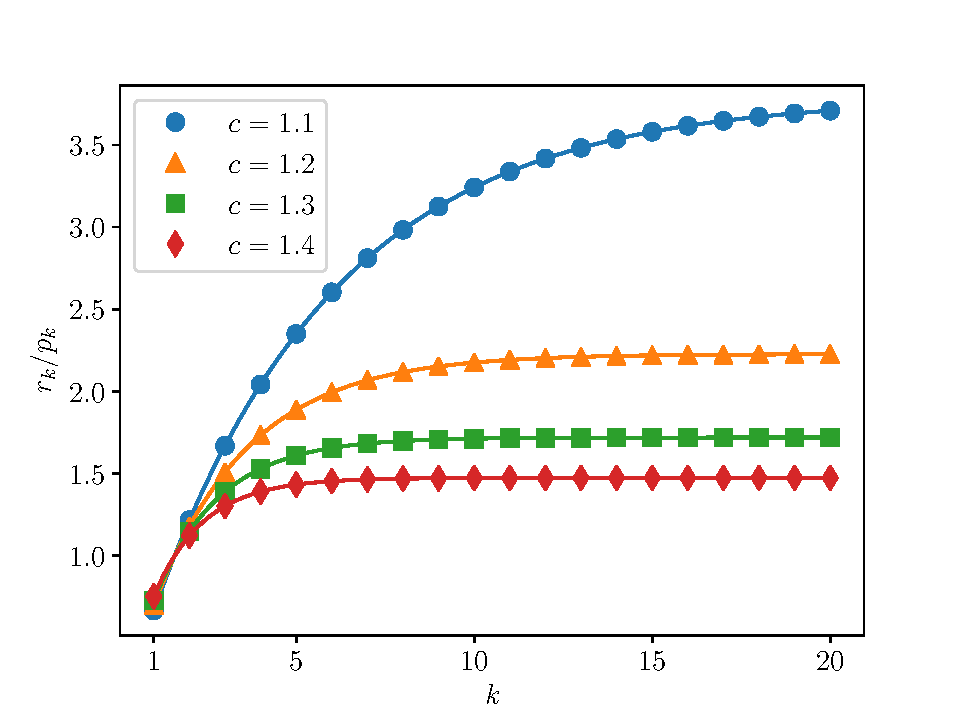
\includegraphics[width=0.8\textwidth]{ER_reconstruction.pdf}
	\caption{Bias factor $r_k/p_k$ for $r_k$ being the degree distribution of the GCC of an Erdos-Renyi network with various mean degree $c$ and cutoff constant $K = 10000$. The $p_k$ have been determined using the algorithm presented in the text. Solid line is the expected value $(1 - u^k)/S$ for the bias factor.}
	\label{Figure: Erdos-Renyi reconstruction}
\end{figure}

\subsection{Real world networks}

As an example of use of the algorithm presented, we apply it to real networks. We choose two by design connected network from the Konect network database \cite{kunegis2013konect}, the powergrid of the western states of the United States and the road network of the state of California\footnote{The codes of the networks in the Konect database are respectively \code{UG} and \code{RO}.}.

The connected degree distribution $r_k$ is taken to be the empirical degree distribution of the real network considered. As a consequence, the cutoff constant $K$ is the maximal degree appearing in the network. Then, to sample the resulting degree distribution $p_k$, we simply take the number of vertex $d_k$ of degree $k$ to be the closest integer to $n p_k$, where $n$ is the total number of nodes. In the examples presented we use $n = 10^7$.

\begin{figure}
	\sidesubfloat[]{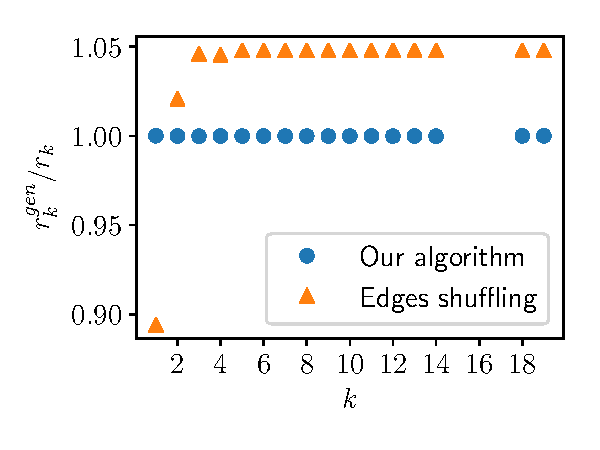
\includegraphics[width=0.45\textwidth]{real_US-power-grid.pdf}}\hfill
	\sidesubfloat[]{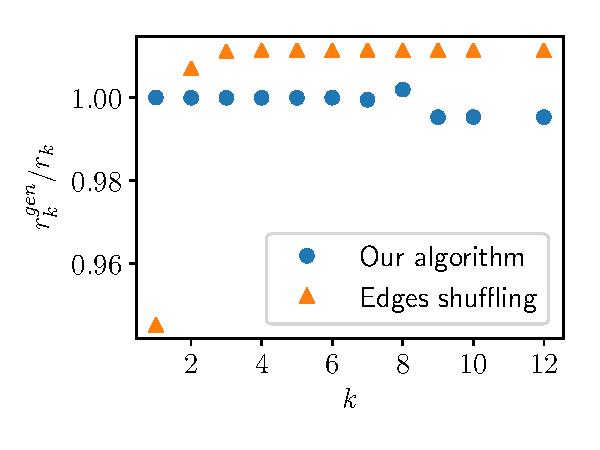
\includegraphics[width=0.45\textwidth]{real_roadNet-CA.pdf}}
	\caption{Plot of the ratio of the generated connected degree distribution $r^{gen}_k$ to the target degree distribution $r_k$ taken from a real network for our algorithm and the edges shuffling method. Missing values correspond to degree with probability $0$ to appear. (a) Western US power-grid network. (b) California road network.}
	\label{Figure: Real examples}
\end{figure}

We compare the degree distribution $r^{gen}_k$ of the GCC of the newly generated network with the target distribution $r_k$ by looking at the ratio $r^{gen}_k / r_k$. Resulting ratios are shown in fig. \ref{Figure: Real examples}, together with the results obtained by taking the GCC of the reshuffled network.

\section{Discussion}

We first quantified the bias affecting the degree distribution of the GCC of a network, compared to the degree distribution of the network as a whole. While small in most case, it becomes significant when a network is close to its critical state.

As a consequence, sampling connected networks with a given degree distribution  by approximated them by the GCC of this degree distribution may introduce undesired biases. To help solve this problem, we introduce an algorithm to determine the degree distribution of a network based on the degree distribution in its GCC. Therefore, it is possible in principle to generate connected network with arbitrary degree distribution, as long as its mean degree is finite.

We then apply the proposed algorithm to classical Erdos-Renyi network, demonstrating that the numerical approximation of the algorithm behaves as expected, despite the imprecisions introduced.

Finally, we apply the algorithm to real world example of network. Comparing it to the edges shuffling method, we can conclude that our algorithm indeed improves it.

\appendix
\section{Convergence of the fixpoint iteration}
\label{Appendix: Fixpoint convergence}

First notice that the case $r_1 = 0$ is trivial, as described in the main text. We will therefore assume in this Appendix that $r_1 > 0$, immediately giving $\mu(0) = r_1 > 0$. Second, not that \eqref{Defition of mu} tells us that $z < 1$ implies $\mu(z) < 1$. From there we separate two cases:

If $u = 1$ is the unique solution of eq. \eqref{Fixpoint equation for u} then $\mu(z)$ must be continuous for $z \in [0, 1]$ and $\mu'(1) < 1$, making $u = 1$ and attractive fixpoint.

On the other hand if there is another solution $u^*$ to eq. \eqref{Fixpoint equation for u}, it is the unique solution with $0 \leq u^* < 1$ since $\mu(z)$ is an increasing function of $z$, as it is demonstrated in Appendix \ref{Appendix: Monotonicity}. Moreover, since $\mu(0) > 0$ we have $\mu'(u^*) < 1$, which makes it an attracting fixpoint and makes $u = 1$ a repulsive one.

We can thus conclude that the fixpoint iteration proposed always converges and converges to the degenerate case $u = 1$ only if it is the unique possibility.

\section{Monotonicity of $\mu(z)$}
\label{Appendix: Monotonicity}

To prove that $\mu(z)$ is an increasing function, we compute its derivative with respect to $z$, which yields
\begin{align}
	\mu'(z) &= \left[\sum_{k = 1}^{\infty}k \pi_k(z)\right]^{-2} \left(s_1(z) + s_2(z)\right) \\
	s_1(z) &= \sum_{j, k}k j \pi_k'(z) \pi_j(z) \left( z^{k-1} -  z^{j-1}\right) \\
	s_2(z) &= \sum_{j, k} k (k - 1) j \pi_k(z) \pi_j(z) z^{k-2}.
\end{align}
The sum $s_1(z)$ can be rewritten as
\begin{align}
	s_1(z) &= \sum_{j > k} k j \left(\pi_k'(z) \pi_j(z) - \pi_j'(z) \pi_k(z)\right) \left(z^{k-1} -  z^{j-1}\right) \\
		&=\sum_{j > k} \frac{k r_k}{1 - z^k} \frac{j r_j}{1 - z^j} \frac{z^k - z^j}{z^2} \left(\frac{k}{z^{-k} - 1} - \frac{j}{z^{-j} - 1}\right)\\
		&=\sum_{j > k} k j \pi_k(z) \pi_j(z) \frac{z^k - z^j}{z^2} \left(\frac{k}{z^{-k} - 1} - \frac{j}{z^{-j} - 1}\right).
\end{align}
Using the fact that the function
\begin{align}
	f_z(\lambda) = \frac{\lambda}{z^{-\lambda} - 1}
\end{align}
is a decreasing function of $\lambda$ we can see that for $z \in [0, 1)$ and $j > k$ we have
\begin{align}
	z^k - z^j &\geq 0 \\
	\frac{k}{z^{-k} - 1} - \frac{j}{z^{-j} - 1} &\geq 0,
\end{align}
and thus $s_1(z) \geq 0$. Moreover each terms in $s_2(z)$ is non-negative, so we have $s_2(z) \geq 0$. We can therefore conclude that $\mu'(z) \geq 0$ and thus that $\mu(z)$ is an increasing function of $z$.

\printbibliography{}

\end{document}